\documentclass[12pt, twoside]{article}
\usepackage[letterpaper, margin=1in, head=30pt, headsep=0.1in]{geometry}
\usepackage[english]{babel}
\usepackage[utf8]{inputenc}
\usepackage{amsmath}
\usepackage{amsfonts}
\usepackage{amssymb}
\usepackage{tikz}
\usetikzlibrary{quotes, angles}

\usepackage{graphicx}
\usepackage{enumitem}
\usepackage{multicol}

%\usepackage{pgfplots}
%\pgfplotsset{width=10cm,compat=1.9}
%\usepgfplotslibrary{statistics}
%\usepackage{pgfplotstable}
%\usepackage{tkz-fct}
%\usepackage{venndiagram}

\usepackage{fancyhdr}
\pagestyle{fancy}
\fancyhf{}
\renewcommand{\headrulewidth}{0pt} % disable the underline of the header
\raggedbottom
\newif\ifmeta
\metatrue %print standards and topics tags

\title{Math AI Worksheet Generator and Formative Assessment System}
\author{Chris Huson}
\date{February 2021}

%\fancyhead[RE]{\thepage}
%\fancyhead[RO]{\thepage \\ Name: \hspace{3cm}}
%\fancyhead[L]{BECA / Dr. Huson / 10th Grade Geometry\\* 7 June 2019}
%
%\begin{document}
%\subsubsection*{13.7 Homework: Cross sections, distance applications}
%\fancyhead[L]{BECA / Dr. Huson / Geometry 03-Volume+angle-bisectors\\* pset ID: 34}

\begin{document}

\subsubsection*{6.4 Prequiz}
\begin{enumerate}

\item Do Now: Use the Graspable Math algebra calculator to substitute and simplify. Show your work in this slide by
\begin{enumerate}
  \item Copy / paste an image (on a Mac, Command-Control-Shift 4 to copy to the clipboard), or
  \item Use the camera tool to upload from your Desktop (Command-Shift 4 on a Mac)
\end{enumerate}

\newpage
\item Find the slope of the line $\overleftrightarrow{AB}$, $A(1,5)$, $B(3,1)$. Use the formula and show the substitution step.
\begin{multicols}{2}
  $\displaystyle m = \frac{y_B - y_A}{x_B - x_A}$
    \vspace{2cm}
    \begin{flushright}
    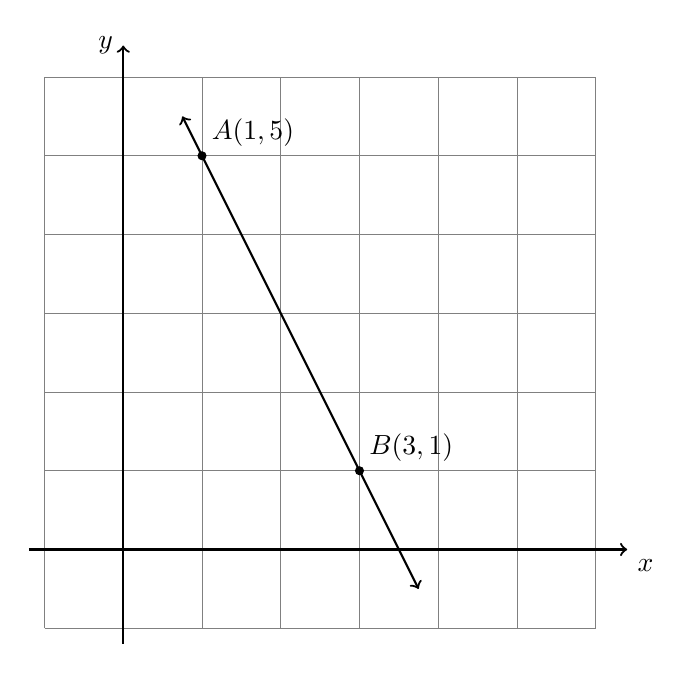
\begin{tikzpicture}[scale=1]
      \draw [help lines] (-1,-1) grid (6,6);
      \draw [thick, ->] (-1.2,0) -- (6.4,0) node [below right] {$x$};
      \draw [thick, ->] (0,-1.2)--(0,6.4) node [left] {$y$};
      \draw [fill] (1,5) circle [radius=0.05] node[above right] {$A(1,5)$};
      \draw [fill] (3,1) circle [radius=0.05] node[above right] {$B(3,1)$};
      \draw [<->, thick] (0.75,5.5)--(3.75,-0.5);
    \end{tikzpicture}
    \end{flushright}
\end{multicols}

\newpage
\item Plot the points and find the slope of the line $\overleftrightarrow{RS}$, $R(1,2)$, $S(4,5)$. Use the formula and show the substitution step. As a check, draw the line and count the rise and run.
\begin{multicols}{2}
  $\displaystyle m = \frac{y_S - y_R}{x_S - x_R}$
    \vspace{2cm}
    \begin{flushright}
    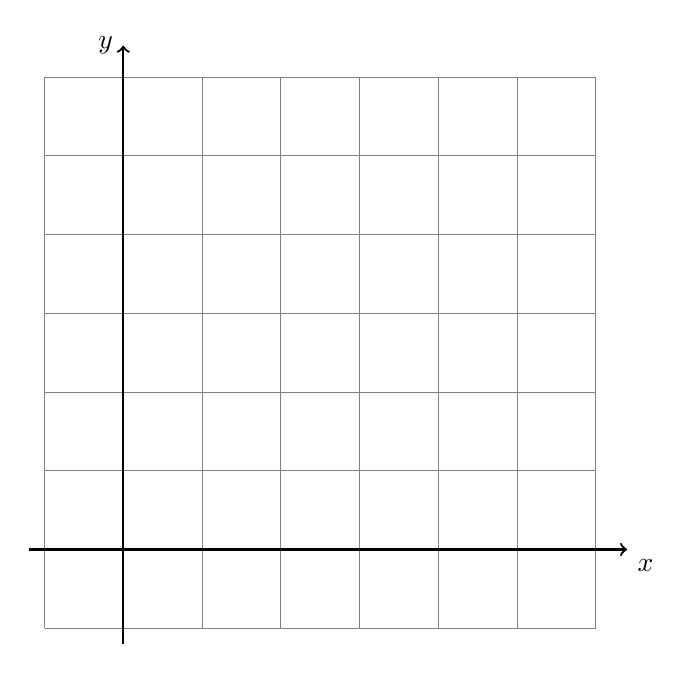
\begin{tikzpicture}[scale=1]
      \draw [help lines] (-1,-1) grid (6,6);
      \draw [thick, ->] (-1.2,0) -- (6.4,0) node [below right] {$x$};
      \draw [thick, ->] (0,-1.2)--(0,6.4) node [left] {$y$};
      %\draw [fill] (2,1) circle [radius=0.05] node[above left] {$A(2,1)$};
      %\draw [fill] (3,4) circle [radius=0.05] node[above right] {$B(3,4)$};
      %\draw [<->, thick] (1,-2)--(4,7);
    \end{tikzpicture}
    \end{flushright}
\end{multicols}

\newpage
\item Find the equation of the given line $\overleftrightarrow{AB}$, $A(0,-1)$, $B(6,3)$.
\begin{multicols}{2}
    \begin{enumerate}[itemsep=1.2cm]
      \item Find the slope, $m$, showing the substitution step in the slope formula: \\[0.25cm]
      $\displaystyle m = (y_B - y_A)/(x_B - x_A)$
      \item Write down the $y$-intercept.
      \item Write the equation of the line.
      \end{enumerate}
    \begin{flushright}
    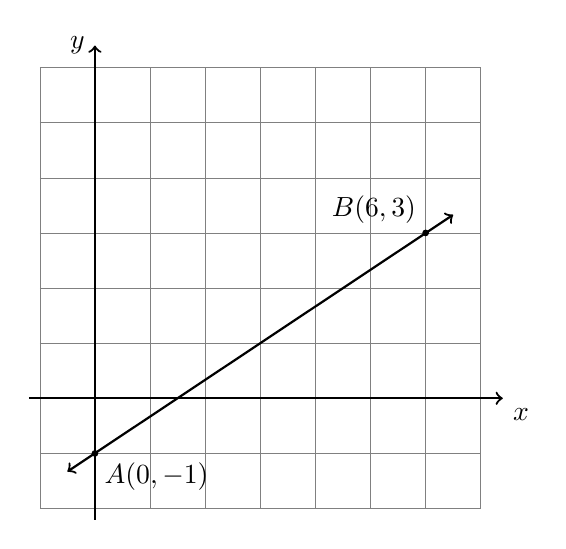
\begin{tikzpicture}[scale=0.7]
      \draw [help lines] (-1,-2) grid (7,6);
      \draw [thick, ->] (-1.2,0) -- (7.4,0) node [below right] {$x$};
      \draw [thick, ->] (0,-2.2)--(0,6.4) node [left] {$y$};
      \draw [fill] (0,-1) circle [radius=0.05] node[below right] {$A(0,-1)$};
      \draw [fill] (6,3) circle [radius=0.05] node[above left] {$B(6,3)$};
      \draw [<->, thick] (-0.5,-1.33)--(6.5,3.33);
    \end{tikzpicture}
    \end{flushright}
\end{multicols}

\newpage
\item Complete each statement about linear equations.
\begin{enumerate}[itemsep=0.5cm]
  \item What is the slope of the line $y = 2x + 3$?
  \item Which has an zero slope, a vertical or horizontal line?
  \item What is the $y$-intercept of the line $y = \frac{1}{2}x$?
  \item What is the slope of a vertical line?
  \item What is the slope of the line $y = -x + 3$?

\end{enumerate}

\newpage
\item Is the point $C(3,1)$ on the line $l: y=-\frac{3}{2}x+5$? \\[0.5cm]
Support your answer with \emph{both} algebra (substitute $C$'s coordinates into the equation) and geometry by graphing the line and point $C$.
  \begin{flushright}
  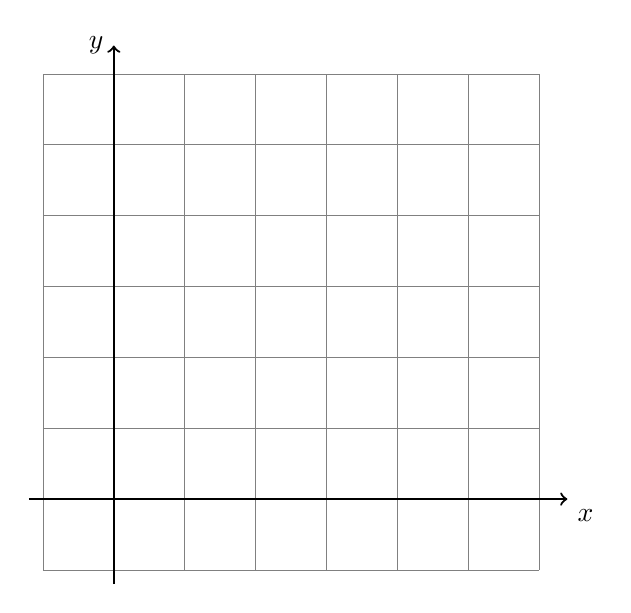
\begin{tikzpicture}[scale=0.9]
    \draw [help lines] (-1,-1) grid (6,6);
    \draw [thick, ->] (-1.2,0) -- (6.4,0) node [below right] {$x$};
    \draw [thick, ->] (0,-1.2)--(0,6.4) node [left] {$y$};
  \end{tikzpicture}
  \end{flushright}

\newpage
\item Two perpendicular lines are shown in the graph, $p$ and $q$. Line $p$ has a slope of $\displaystyle m = \frac{1}{3}$ and a $y$-intercept $b=2$.
\begin{multicols}{2}
    \begin{enumerate}[itemsep=1cm]
      \item Write down the equation of line $p$.
      \item What is the slope of line $q$, $m_\perp$?
      \item Spicy: Line $q$ crosses the $x$-axis at $(4,0)$. What is its $y$-intercept?
      \end{enumerate}
    \begin{flushright}
    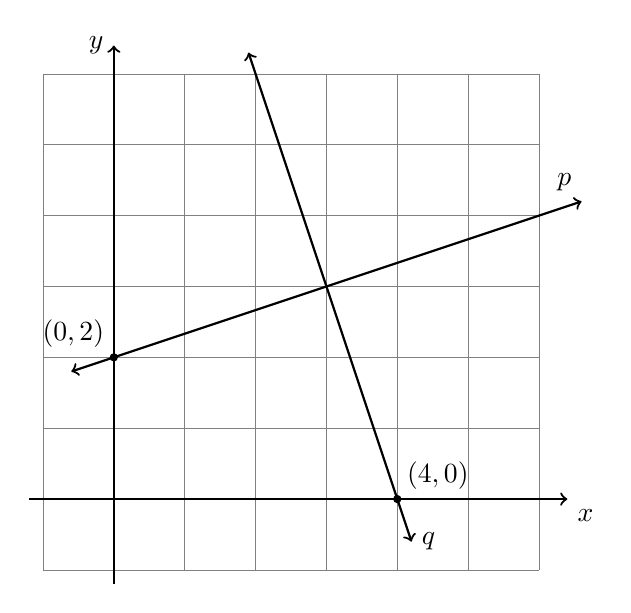
\begin{tikzpicture}[scale=0.9]
      \draw [help lines] (-1,-1) grid (6,6);
      \draw [thick, ->] (-1.2,0) -- (6.4,0) node [below right] {$x$};
      \draw [thick, ->] (0,-1.2)--(0,6.4) node [left] {$y$};
      \draw [fill] (0,2) circle [radius=0.05] node[above left] {$(0,2)$};
      \draw [fill] (4,0) circle [radius=0.05] node[above right] {$(4,0)$};
      \draw [<->, thick] (-0.6,1.8)--(6.6,4.2) node [above left]{$p$};
      \draw [<->, thick] (1.9,6.3)--(4.2,-0.6) node [right]{$q$};
    \end{tikzpicture}
    \end{flushright}
\end{multicols}

\newpage
\item Write down the slope perpendicular to each slope (its negative reciprocal).
\begin{enumerate}[itemsep=0.9cm]
  \item If $m = -2$ then $m_{\perp}=$
  \item If $\displaystyle m = -\frac{5}{4}$ then $m_{\perp}=$
  \item If $m = 1$ then $m_{\perp}=$
  \item If $\displaystyle m = \frac{3}{1}$ then $m_{\perp}=$
\end{enumerate}

\newpage
\item $\triangle ABC$ with vertices $A(-1,6)$, $B(4,1)$, and $C(5,4)$ is shown. \\[0.5cm]
Find the slopes of $\overleftrightarrow{AC}$ and $\overleftrightarrow{BC}$. Is the triangle a right triangle? Justify your answer.
  \begin{flushright}
    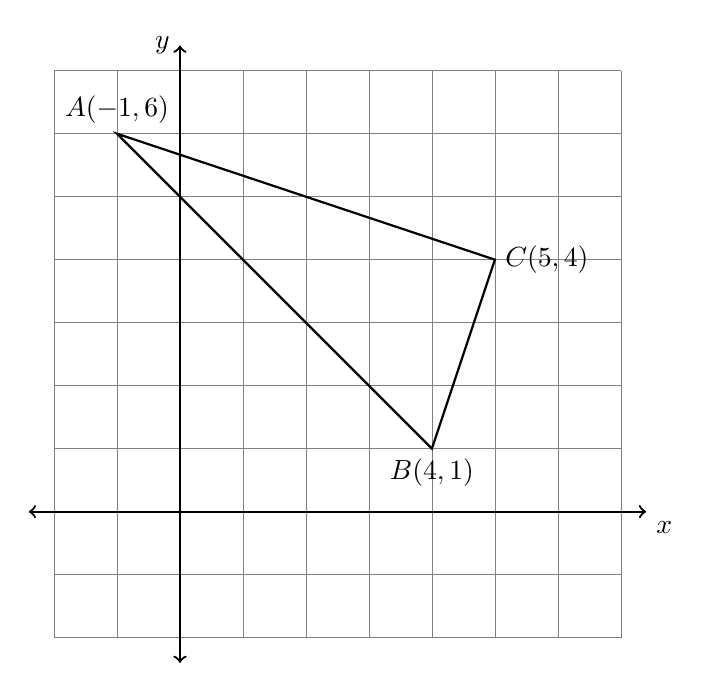
\begin{tikzpicture}[scale=0.8]
      \draw [help lines] (-2,-2) grid (7,7);
      \draw [thick, <->] (-2.4,0) -- (7.4,0) node [below right] {$x$};
      \draw [thick, <->] (0,-2.4)--(0,7.4) node [left] {$y$};
      \draw [thick] (-1,6) node[above] {$A(-1,6)$}--
        (5,4) node[right] {$C(5,4)$}--
        (4,1) node[below] {$B(4,1)$}--
        cycle;
    \end{tikzpicture}
    \end{flushright}

\newpage
\item Plot a right triangle using Geogebra/classic (use the grid). Paste an image of your work in this Classkick slide from the clipboard or by using the ``camera'' tool.\\[0.25cm]
Spicy: Show the measures the slopes of the triangle legs and the measure of the right angle.

    
\end{enumerate}
\end{document}

\newpage
\item A point labeled $C$ and vector $(1,3)$ are shown Geogebra/classic. Identify the following objects and tools.
  \begin{enumerate}
    \item Circle the vector
    \item Make an ``X'' where to click for the menu ``Name \& Value'' that will label point $C$ as an ordered pair.
    \item Mark with an arrow the menu where the ``Translate by vector'' tool is found.
  \end{enumerate}
  \begin{flushright}
    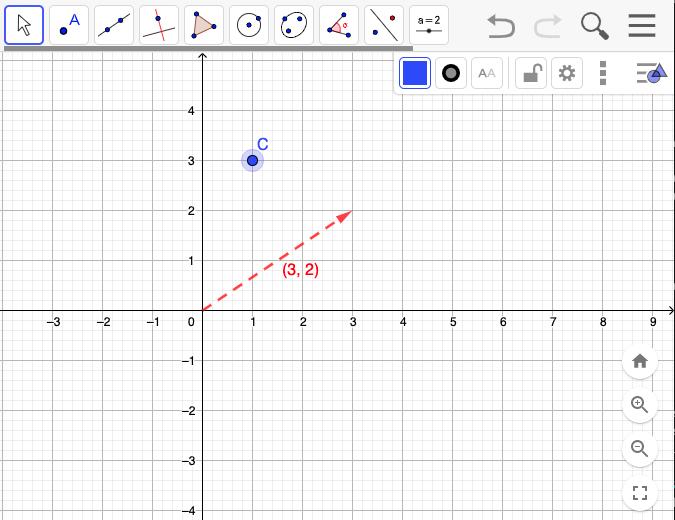
\includegraphics[width=6in]{5-11Geogebra_toolbar.png}
  \end{flushright}
